\documentclass{article}
\usepackage[utf8]{inputenc}
\usepackage{graphicx}
\usepackage{amsfonts, amssymb, amsmath}
\usepackage{float}
\usepackage{fancyhdr}
\usepackage{geometry}  
\usepackage{lastpage} % obtenir le nombre total de page
\usepackage{titlesec} % permet de modifier la taille des sections 


\geometry{landscape, margin=1in}
\parindent 0px
\titleformat{\section}{\huge\bfseries}{\thesection}{0.5em}{}
\titleformat{\subsection}{\huge\bfseries}{\thesubsection}{0.5em}{}

\fancypagestyle{landscape}{
    \fancyhf{}
    \renewcommand{\headrulewidth}{0.5pt}
    \renewcommand{\footrulewidth}{0.5pt} 
    \fancyfoot[R]{\thepage /\pageref{LastPage}}
    \fancyfoot[L]{\leftmark \, - \rightmark}
}


\title{Comment modéliser avec une approche réaliste de l’eau dans un jeu vidéo ?}
\author{Fortier Benjamin - Posez Bastien}
\date{\today}



\begin{document}
\huge
\thispagestyle{landscape}
\maketitle


\newpage
\thispagestyle{landscape}
\vspace*{2pt}
\textbf{Mise en contexte:}
\begin{center}
    L’industrie du jeu qui ne fait que de se développer, la présence de réalisme au sein de nouveaux jeux est un argument marketing important qui permet de faciliter l’immersion des joueurs. 
\end{center}

\newpage
\thispagestyle{landscape}
\vspace*{\fill}
\begin{center}
    \textbf{Problématique : Comment modéliser avec une approche réaliste de l’eau dans un jeu vidéo ?}    
\end{center}
\vspace*{\fill}

\newpage
\thispagestyle{landscape}
\vspace*{\fill}
\textbf{Objectifs :}
\begin{center}
    \begin{itemize}
        \item Étudier le comportement d’un fluide à l’aide des équations de Navier-Stokes et l’impact des différentes forces sur chaque particule
        \item Réussir à créer une modélisation de fluide grâce à un système de particules
        \item Comprendre l’utilisation d’une fonction Kernel afin de limiter le nombre de calcul
        \item Limiter un maximum la complexité du programme en proposant dans le pire des cas un O(n²)
        \item Créer en premier lieu un rendu 2D puis par la suite un rendu 3D
    \end{itemize}
\end{center}
\vspace*{\fill}


\newpage
\thispagestyle{landscape}

\renewcommand{\contentsname}{\huge Plan :}
\tableofcontents


\newpage
\thispagestyle{landscape}

\section{Modélisation du fluide à l’aide d’un système de particule}
\subsection{Caractéristiques\,\,de\,\,chaque\,\,particule}
\begin{center}
    \includegraphics[width=0.9\textwidth]{Modélisation d'un fluide.png}
\end{center}



\newpage
\thispagestyle{landscape}

\begin{center}
    Deux méthodes distinctes pour modéliser un fluide : 
\end{center}
\parbox{0.5\textwidth}{
    \centering
    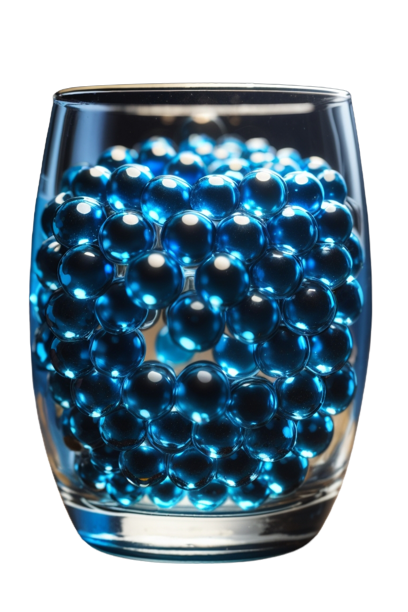
\includegraphics[width=0.3\textwidth]{verre_particule.png}
    \\Méthode des particules
}
\vspace{\fill}

\newpage
\vspace*{2pt}
\thispagestyle{landscape}
On va donc ici choisir un système composé de particules
\vspace*{\fill}
\parbox{0.7\textwidth}{
}
\parbox{0.3\textwidth}{
    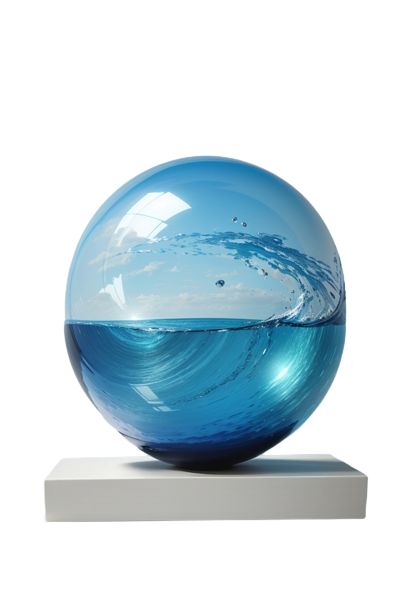
\includegraphics[width=0.3\textwidth]{particule}
    \vspace*{\fill}
}


\newpage
\vspace*{2pt}
\thispagestyle{landscape}
\parbox{0.7\textwidth}{
On va donc ici choisir un système composé de particules
\\Chaque particule  de notre système est définie par : 
}
\parbox{0.3\textwidth}{
    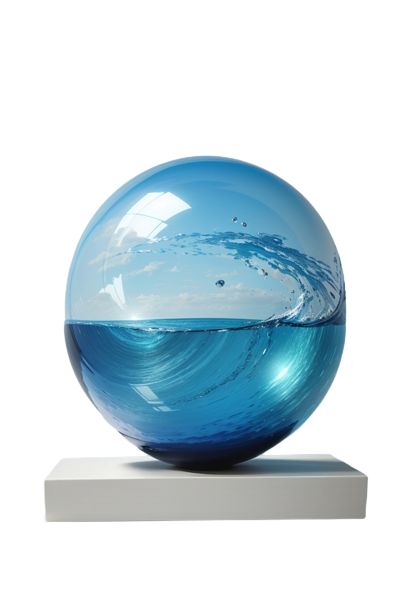
\includegraphics[width=0.3\textwidth]{particule}
}
\vspace*{\fill}

\newpage
\vspace*{2pt}
\thispagestyle{landscape}
\parbox{0.7\textwidth}{
On va donc ici choisir un système composé de particules
\\Chaque particule  de notre système est définie par : 
\\Des paramètres qui sont propres à chaque particule :
}
\parbox{0.3\textwidth}{
    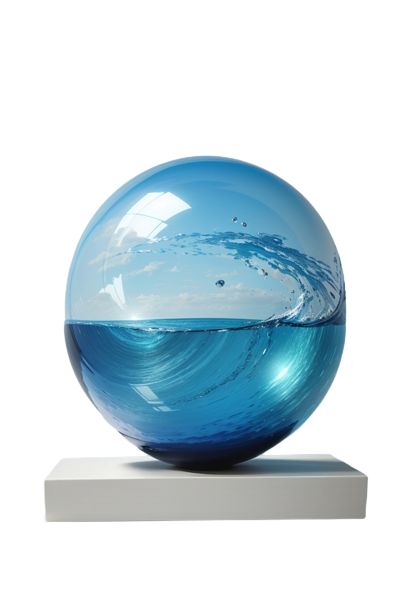
\includegraphics[width=0.3\textwidth]{particule}
}
\vspace*{\fill}



\newpage
\vspace*{2pt}
\thispagestyle{landscape}
\parbox{0.7\textwidth}{
On va donc ici choisir un système composé de particules
\\Chaque particule  de notre système est définie par : 
\\Des paramètres qui sont propres à chaque particule :
\begin{itemize}
    \item Sa position selon l’axe x et l’axe y
    \item Sa vitesse selon l’axe x et l’axe y
    \item Sa direction 
    \item Sa densité
\end{itemize}


Des paramètres qui restent inchangés pour chacune de nos particules : 
}
\parbox{0.3\textwidth}{
    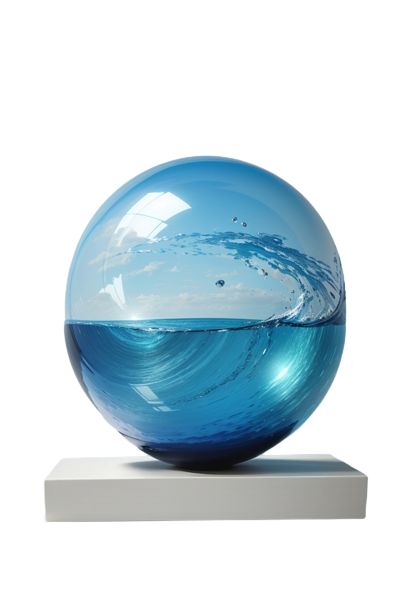
\includegraphics[width=0.3\textwidth]{particule}
}
\vspace*{\fill}

\newpage
\vspace*{2pt}
\thispagestyle{landscape}
\parbox{0.7\textwidth}{
On va donc ici choisir un système composé de particules
\\Chaque particule  de notre système est définie par : 
\\Des paramètres qui sont propres à chaque particule :
\begin{itemize}
    \item Sa position selon l’axe x et l’axe y
    \item Sa vitesse selon l’axe x et l’axe y
    \item Sa direction 
    \item Sa densité
\end{itemize}


Des paramètres qui restent inchangés pour chacune de nos particules : 
\begin{itemize}
    \item Le rayon et la masse
\end{itemize}
}
\parbox{0.3\textwidth}{
    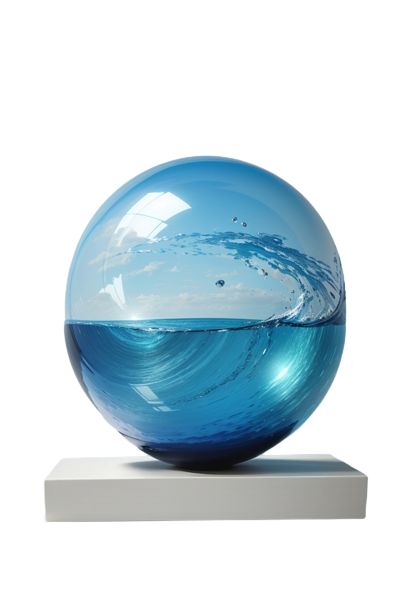
\includegraphics[width=0.3\textwidth]{particule}
}
\vspace*{\fill}

\newpage
\vspace*{2pt}
\thispagestyle{landscape}
\subsection{Collision entre particules}
On considère ici des collisions élastiques entre chaque particule : 
\begin{center}
    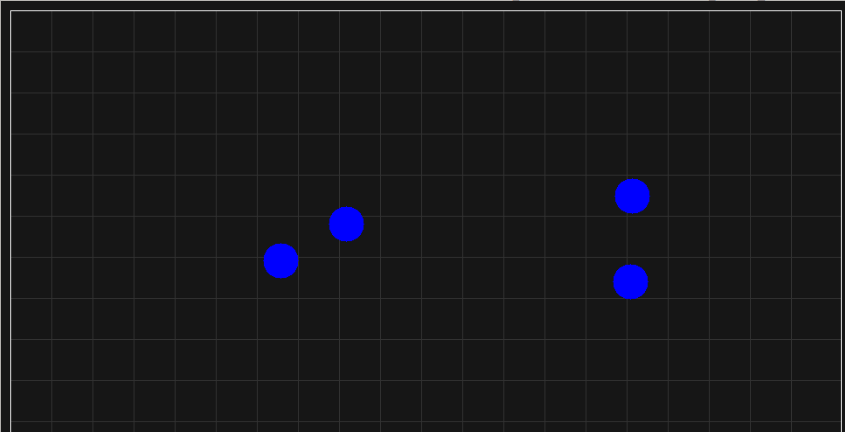
\includegraphics[width=0.9\textwidth]{CollisionP1.png}
\end{center}

\newpage
\vspace*{2pt}
\thispagestyle{landscape}
\textbf{Système de collision}
\\On considère ici des collisions élastiques entre chaque particule : 
\begin{center}
    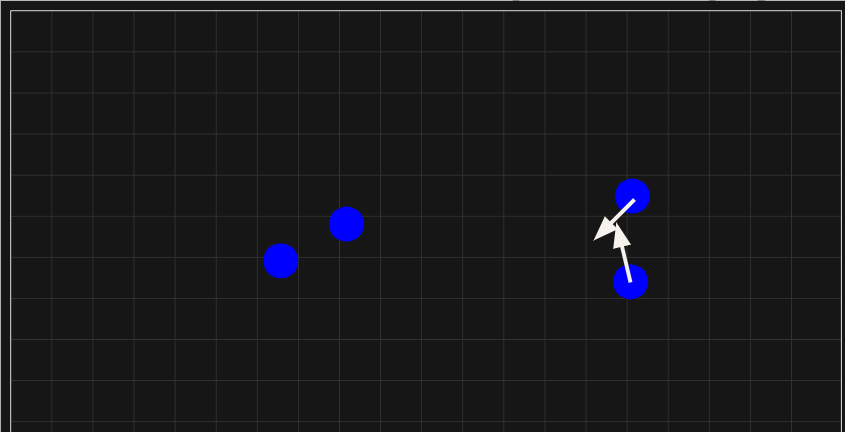
\includegraphics[width=0.9\textwidth]{CollisionP2.png}
\end{center}

\newpage
\vspace*{2pt}
\thispagestyle{landscape}
\textbf{Système de collision}
\\[2ex]On considère ici des collisions élastiques entre chaque particule : 
\begin{center}
    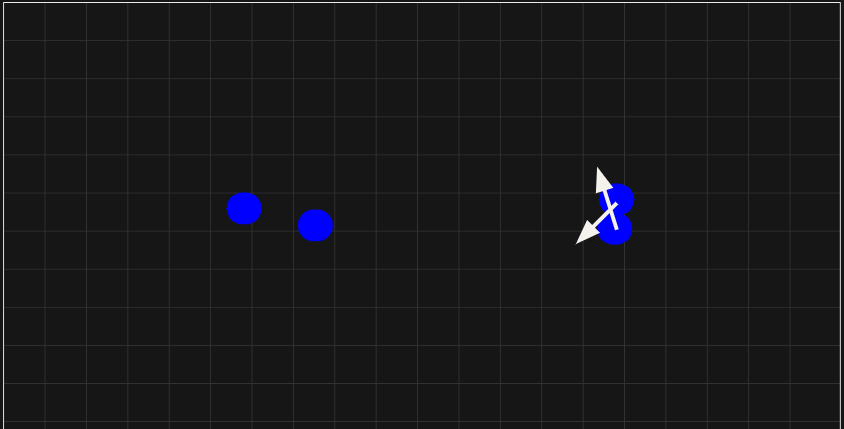
\includegraphics[width=0.9\textwidth]{CollisionP3.png}
\end{center}

\newpage
\vspace*{2pt}
\thispagestyle{landscape}
\textbf{Système de collision}
\\On considère ici des collisions élastiques entre chaque particule : 
\begin{center}
    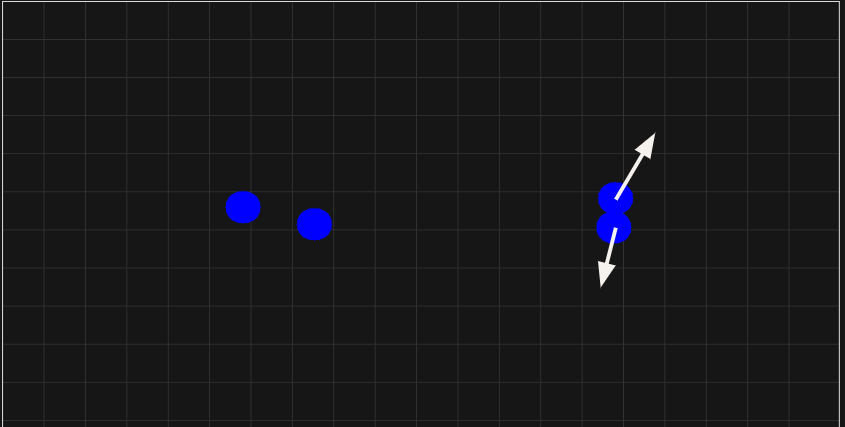
\includegraphics[width=0.9\textwidth]{CollisionP4.png}
\end{center}

\newpage
\vspace*{2pt}
\thispagestyle{landscape}
\textbf{Système de collision}
\\On considère ici des collisions élastiques entre chaque particule : 
\begin{center}
    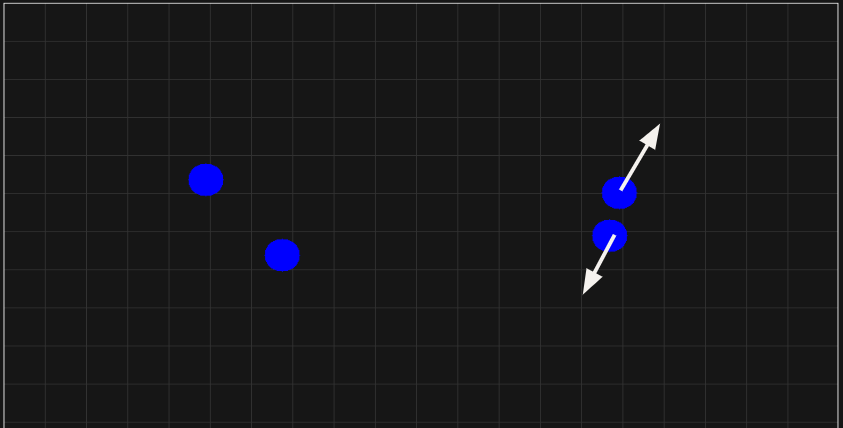
\includegraphics[width=0.9\textwidth]{CollisionP5.png}
\end{center}


\newpage
\vspace*{2pt}
\thispagestyle{landscape}
\subsection{Collision avec les bordures}
De plus on considère aussi les collisions comme élastiques entre une particule et un mur : \\[64pt]
\parbox{0.25\textwidth}{
    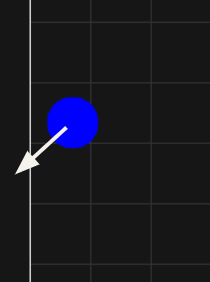
\includegraphics[width=0.20\textwidth]{CollisionM1.png}
}


\newpage
\vspace*{2pt}
\thispagestyle{landscape}
\textbf{Système de collision}\\
De plus on considère aussi les collisions comme élastiques entre une particule et un mur : \\[64pt]
\parbox{0.25\textwidth}{
    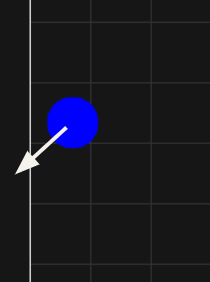
\includegraphics[width=0.20\textwidth]{CollisionM1.png}
}
\parbox{0.25\textwidth}{
    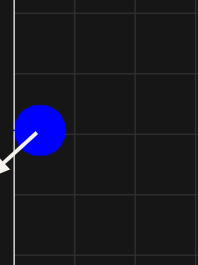
\includegraphics[width=0.20\textwidth]{CollisionM2.png}
}

\newpage
\vspace*{2pt}
\thispagestyle{landscape}
\textbf{Système de collision}\\
De plus on considère aussi les collisions comme élastiques entre une particule et un mur : \\[64pt]
\parbox{0.25\textwidth}{
    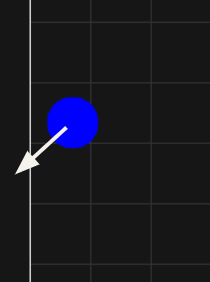
\includegraphics[width=0.20\textwidth]{CollisionM1.png}
}
\parbox{0.25\textwidth}{
    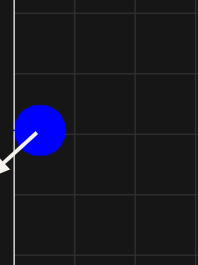
\includegraphics[width=0.20\textwidth]{CollisionM2.png}
}
\parbox{0.25\textwidth}{
    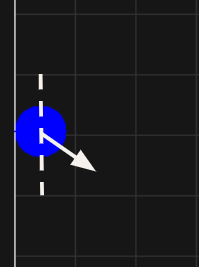
\includegraphics[width=0.20\textwidth]{CollisionM3.png}
}


\newpage
\vspace*{2pt}
\thispagestyle{landscape}
\textbf{Système de collision}\\
De plus on considère aussi les collisions comme élastiques entre une particule et un mur : \\[64pt]
\parbox{0.25\textwidth}{
    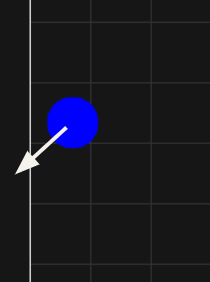
\includegraphics[width=0.20\textwidth]{CollisionM1.png}
}
\parbox{0.25\textwidth}{
    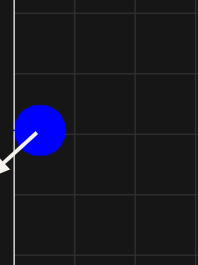
\includegraphics[width=0.20\textwidth]{CollisionM2.png}
}
\parbox{0.25\textwidth}{
    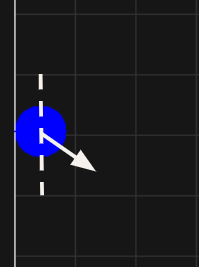
\includegraphics[width=0.20\textwidth]{CollisionM3.png}
}
\parbox{0.25\textwidth}{
    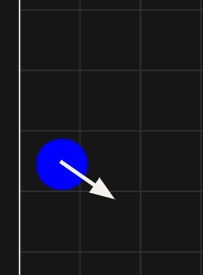
\includegraphics[width=0.20\textwidth]{CollisionM4.png}
}

\newpage
\vspace*{2pt}
\thispagestyle{landscape}
\section{Résolution numérique des équations de Navier-Stokes}
\begin{center}
    \includegraphics*{NavierStokes.png}
\end{center}

\newpage
\vspace*{2pt}
\thispagestyle{landscape}
\begin{center}
    Équations de Navier-Stokes
    $$\frac{dv}{dt} = -\nabla p + \rho g + \mu \nabla ^2 v$$
\end{center}

\newpage
\vspace*{2pt}
\thispagestyle{landscape}
\begin{center}
    Équations de Navier-Stokes
    $$\frac{dv}{dt} = -\nabla p + \rho g + \mu \nabla ^2 v$$
\end{center}
\begin{itemize}
    \item $-\nabla p $ : Force de pression
\end{itemize}

\newpage
\vspace*{2pt}
\thispagestyle{landscape}
\begin{center}
    Équations de Navier-Stokes
    $$\frac{dv}{dt} = -\nabla p + \rho g + \mu \nabla ^2 v$$
\end{center}
\begin{itemize}
    \item $-\nabla p $ : Force de pression
    \item $ \rho g $ : Forces extérieures
\end{itemize}

\newpage
\vspace*{2pt}
\thispagestyle{landscape}
\begin{center}
    Équations de Navier-Stokes
    $$\frac{dv}{dt} = -\nabla p + \rho g + \mu \nabla ^2 v$$
\end{center}
\begin{itemize}
    \item $-\nabla p $ : Force de pression
    \item $ \rho g $ : Forces extérieures
    \item $\mu \nabla ^2 v$ : Force de viscosité
\end{itemize}





\newpage
\vspace*{2pt}
\thispagestyle{landscape}
\subsection{Force de pression}
Calcul numérique de la force de pression s’exerçant sur chaque particule :

$$ f^{pressure}_i = -\nabla p(r_i) = - \Sigma_j m_j \frac{p_j}{\rho_j} \nabla W(r_i-r_{j,h}).$$
Avec : 
$$p = k (\rho - \rho_0)$$

\newpage
\vspace*{2pt}
\thispagestyle{landscape}
\subsection{Force de pression}
Calcul numérique de la force de pression s’exerçant sur chaque particule :

$$ f^{pressure}_i = -\nabla p(r_i) = - \Sigma_j m_j \frac{p_j}{\rho_j} \nabla W(r_i-r_{j,h}).$$
Avec : 
$$p = k (\rho - \rho_0)$$
Et la fonction Kernel: 
$$\nabla W(r_i-r_{j,h})$$

\newpage
\vspace*{2pt}
\thispagestyle{landscape}
\subsection{Force de viscosité}
\parbox{0.34\textwidth}{
    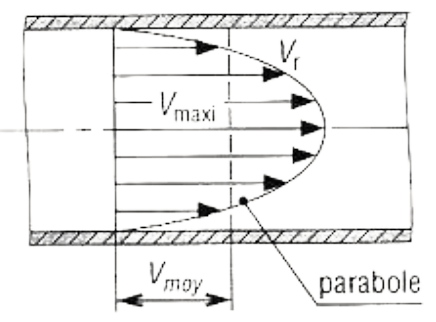
\includegraphics[width=0.35\textwidth]{visco.png}
}
\parbox{0.33\textwidth}{
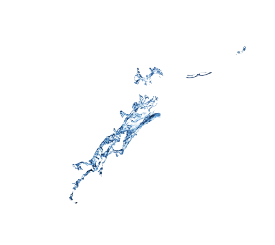
\includegraphics[width=0.35\textwidth]{visco_eau.png}
\vspace*{2pt}
\begin{center}
    Coefficient de viscosité de l’eau : 
    $1$x$10^{-3} Pa.s$
\end{center}
}
\parbox{0.33\textwidth}{
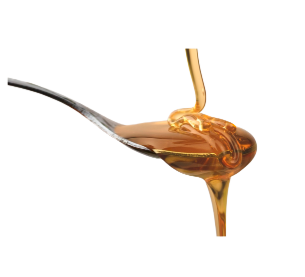
\includegraphics[width=0.35\textwidth]{visco_miel.png}
\vspace*{2pt}
\begin{center}
    Coefficient de viscosité du miel : 
    $10000 Pa.s$
\end{center}
}

\newpage
\vspace*{2pt}
\thispagestyle{landscape}
Calcul numérique de la viscosité s’exerçant sur chaque particule :
$$ f^{viscosite}_i = \mu \Sigma m_j \frac{v_j-v_i}{\rho_j} \nabla ^2 W(r_i- r_{j,h}).$$

\newpage
\vspace*{2pt}
\thispagestyle{landscape}
Calcul numérique de la viscosité s’exerçant sur chaque particule :
$$ f^{viscosite}_i = \mu \Sigma m_j \frac{v_j-v_i}{\rho_j} \nabla ^2 W(r_i- r_{j,h}).$$
\begin{itemize}
    \item $\mu$ : viscosité dynamique du fluide 
\end{itemize}

\newpage
\vspace*{2pt}
\thispagestyle{landscape}
Calcul numérique de la viscosité s’exerçant sur chaque particule :
$$ f^{viscosite}_i = \mu \Sigma m_j \frac{v_j-v_i}{\rho_j} \nabla ^2 W(r_i- r_{j,h}).$$
\begin{itemize}
    \item $\mu$ : viscosité dynamique du fluide 
    \item $\nabla ^2 W(r_i- r_{j,h})$ : Laplacien du noyau 
\end{itemize}

\newpage
\vspace*{2pt}
\thispagestyle{landscape}
Pour le calcul de nabla ($\nabla$) :
$$\vec{grad} f = \vec{\nabla} f = (\frac{\partial f}{\partial x}\,\,\,\,\frac{\partial f}{\partial y}\,\,\,\,\frac{\partial f}{\partial z})$$

\newpage
\vspace*{2pt}
\thispagestyle{landscape}
\subsection{Calcul numérique de dérivée partielle}
Méthode des différences finies centrées pour calculer des dérivées partielle numériquement :\\
$$ \frac{u(x+h)-u(x-h)}{2h} = u'(x)+\frac{h^2}{6}u^{(3)}(x)+h^2 \epsilon_3(h) \approx u'(x)$$
$$\frac{u(x+2h)-2u(x+h)+u(x)}{h^2} = u''(x)+hu^{(3)}(x)+h\epsilon_3(h) \approx u''(x)$$



\newpage
\vspace*{2pt}
\thispagestyle{landscape}
\section{Optimisation des algorithmes}
\begin{center}
    
\includegraphics{Optimisation.png}
\end{center}


\newpage
\vspace*{2pt}
\thispagestyle{landscape}
\subsection{Utilisation de la fonction Kernel}
Utilisation d’une fonction Kernel pour limiter le nombre d’opérations : 

\begin{itemize}
    \item Si la distance entre les deux particules $r$ est telle que $0 \leq r \leq h$ alors $W > 0$
    \item Si $r > h$ alors $W = 0$
\end{itemize}
\begin{center}
    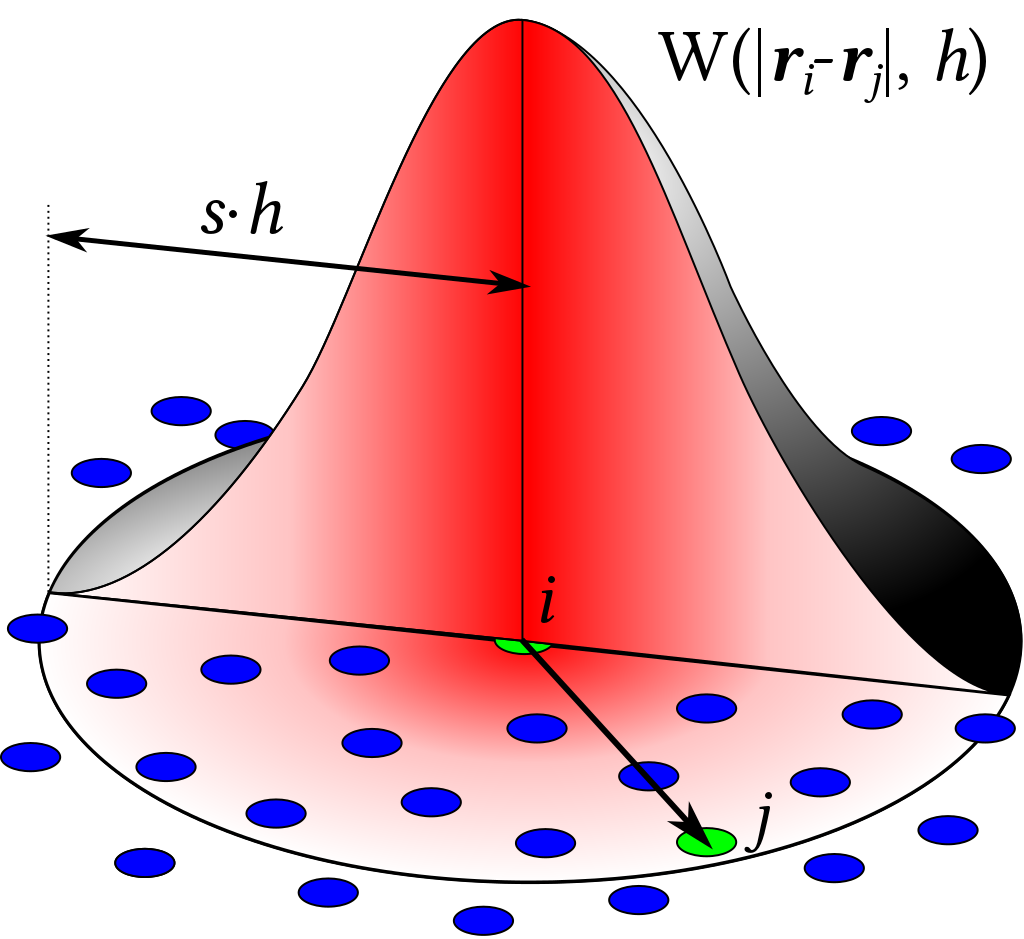
\includegraphics[width=0.4\textwidth]{fonction_kernel.png}
\end{center}

\newpage
\vspace*{2pt}
\thispagestyle{landscape}
\subsection{Utilisation de la fonction Kernel}
Utilisation d’une fonction Kernel pour limiter le nombre d’opérations :\\
La valeur du kernel pour la  force de pression est égal à :\\
$$W_{pression}(r,h)= \frac{15}{\pi h^6}$$ 
La valeur du kernel pour la viscosité est égale à:
$$W_{viscosite}(r,h)= \frac{15}{2\pi h^3}$$

\newpage
\vspace*{2pt}
\thispagestyle{landscape}
\begin{center}
    \section{Résultat}
    
\includegraphics[width=0.5\textwidth]{result.png}
\end{center}



\newpage
\vspace*{2pt}
\thispagestyle{landscape}
\subsection{Affichage}
Résultats du programme : Pour 625 particules 
\begin{center}
    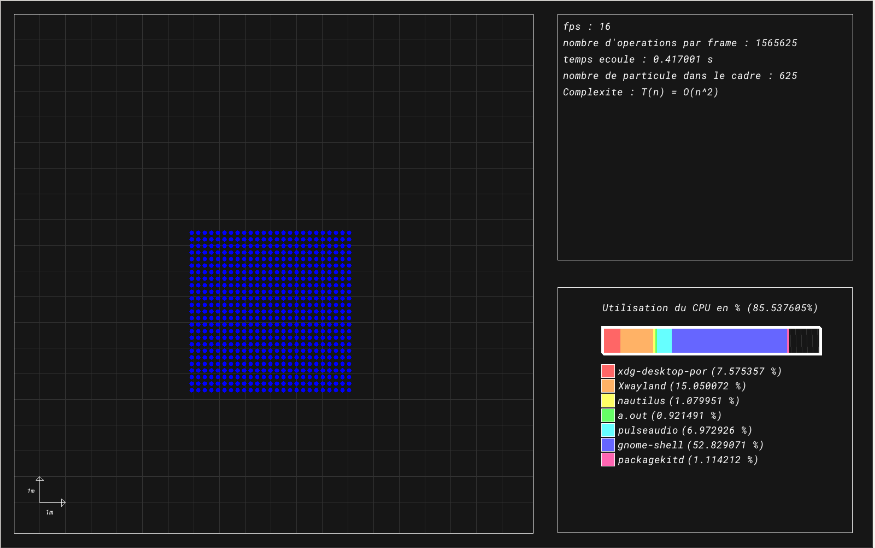
\includegraphics[width=0.9\textwidth]{R_Frame1.png}
\end{center}

\newpage
\vspace*{2pt}
\thispagestyle{landscape}
Résultats du programme : Pour 625 particules 
\begin{center}
    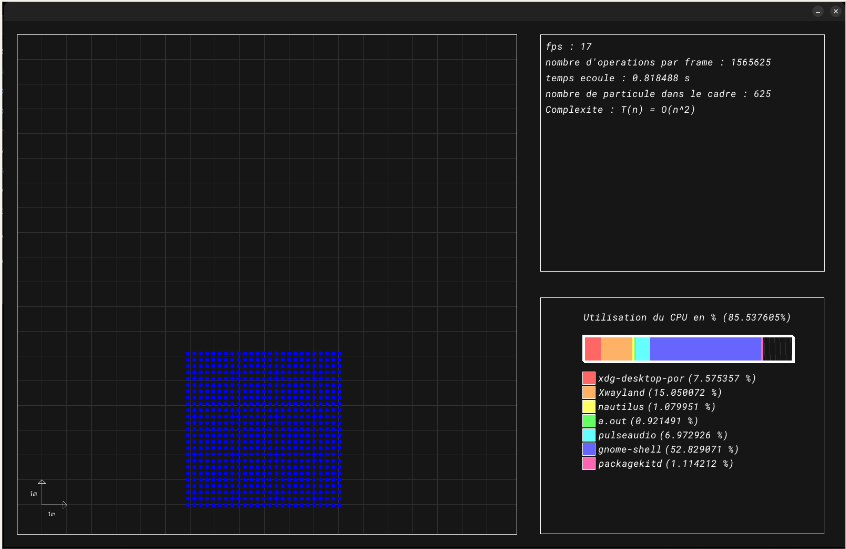
\includegraphics[width=0.9\textwidth]{R_Frame2.png}
\end{center}

\newpage
\vspace*{2pt}
\thispagestyle{landscape}
Résultats du programme : Pour 625 particules 
\begin{center}
    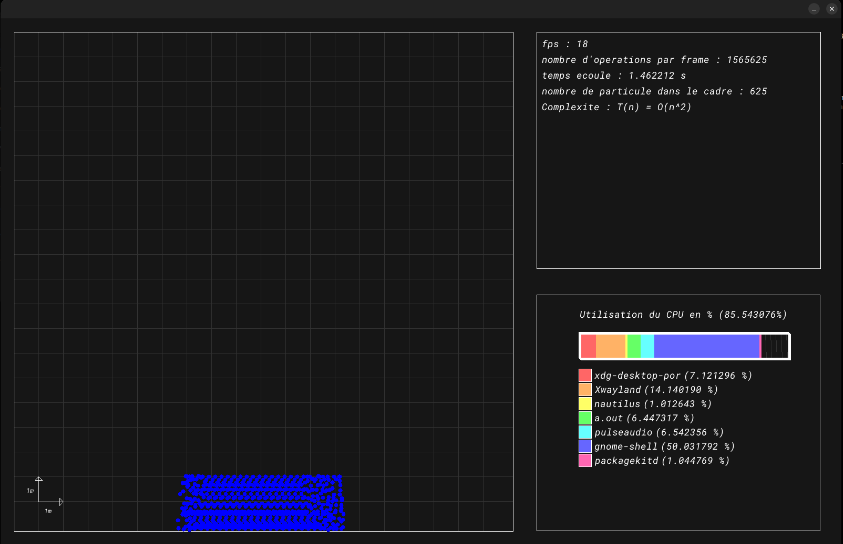
\includegraphics[width=0.9\textwidth]{R_Frame3.png}
\end{center}

\newpage
\vspace*{2pt}
\thispagestyle{landscape}
Résultats du programme : Pour 625 particules 
\begin{center}
    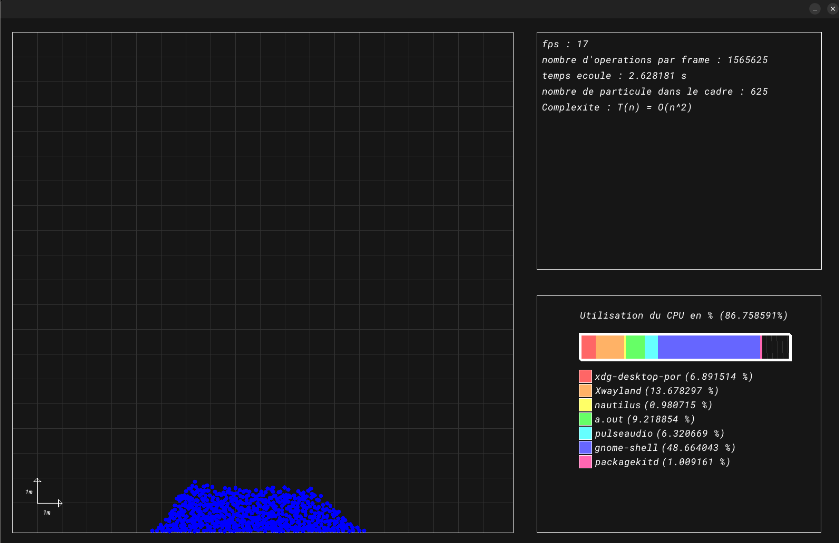
\includegraphics[width=0.9\textwidth]{R_Frame4.png}
\end{center}

\newpage
\vspace*{2pt}
\thispagestyle{landscape}
Résultats du programme : Pour 625 particules 
\begin{center}
    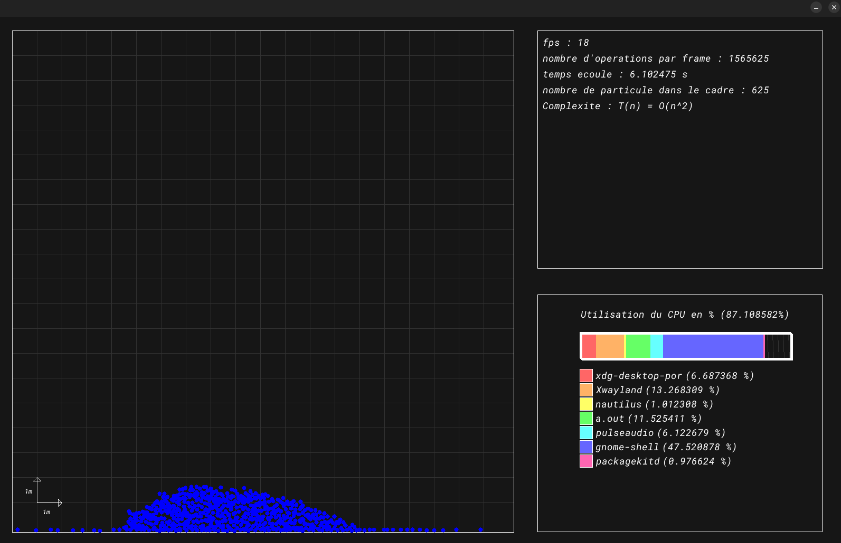
\includegraphics[width=0.9\textwidth]{R_Frame5.png}
\end{center}

\newpage
\vspace*{2pt}
\thispagestyle{landscape}
Résultats du programme : Pour 625 particules 
\begin{center}
    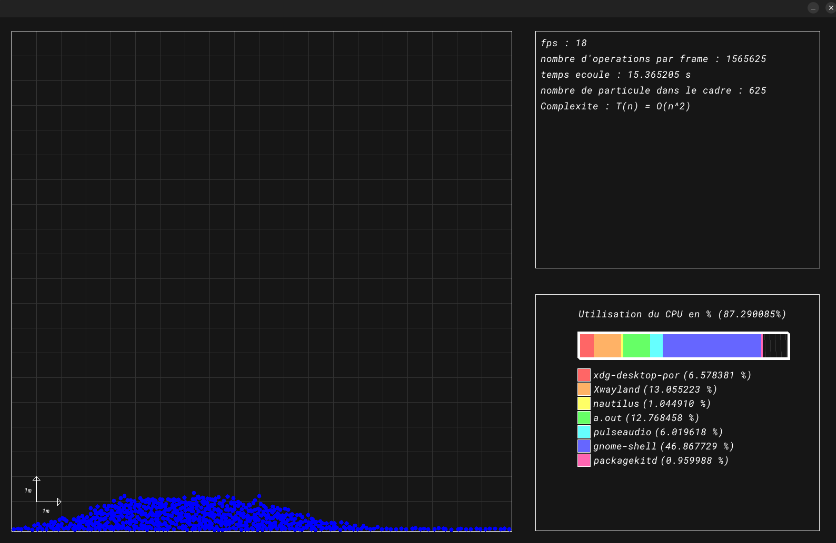
\includegraphics[width=0.9\textwidth]{R_Frame6.png}
\end{center}

\newpage
\vspace*{2pt}
\thispagestyle{landscape}
\subsection{Performance}
Pour notre simulation avec 625 particules, on a les statistiques suivantes  :
\begin{itemize}
    \item Une complexité en 0(n²) avec environ 1 500 000 calculs par image
    \item Une moyenne de 30 fps 
    \item Une utilisation du CPU d’environ 25 % par le programme 
\end{itemize}

\newpage
\vspace*{2pt}
\thispagestyle{landscape}
\textbf{Objectifs futurs :}
\begin{itemize}
    \item Ajout de nouvelles forces (force de tension de surfacique ,   … )
    \item Réaliser un rendu en 3D
    \item Diminuer le nombre de calcul par image en optimisant le programme
\end{itemize}

\newpage
\vspace*{2pt}
\thispagestyle{landscape}
\vspace{\fill}
\begin{center}
    \Huge
    \textbf{Merci de nous avoir écouté}
\end{center}
\vspace{\fill}




\end{document}

